% ---------------------------------------------------------------------------- %
\begin{figure}
	\centering
	\subfigure[\label{fig:linguometer:technical:isd:example:1}]
	{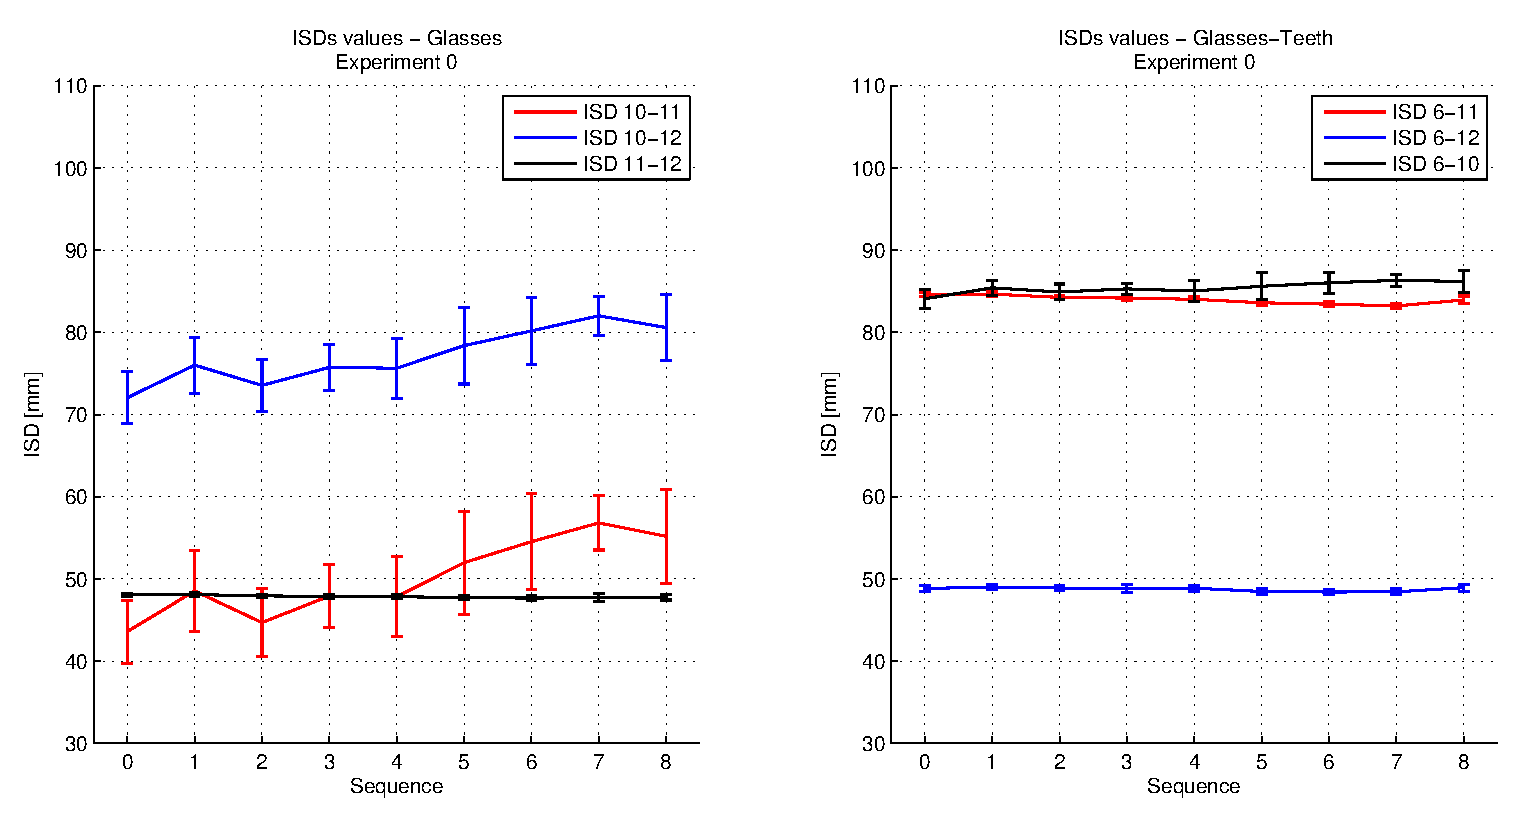
\includegraphics[width=0.75\textwidth]{include/linguometer/images/example_isd_0.eps}}
	\subfigure[\label{fig:linguometer:technical:isd:example:2}]
	{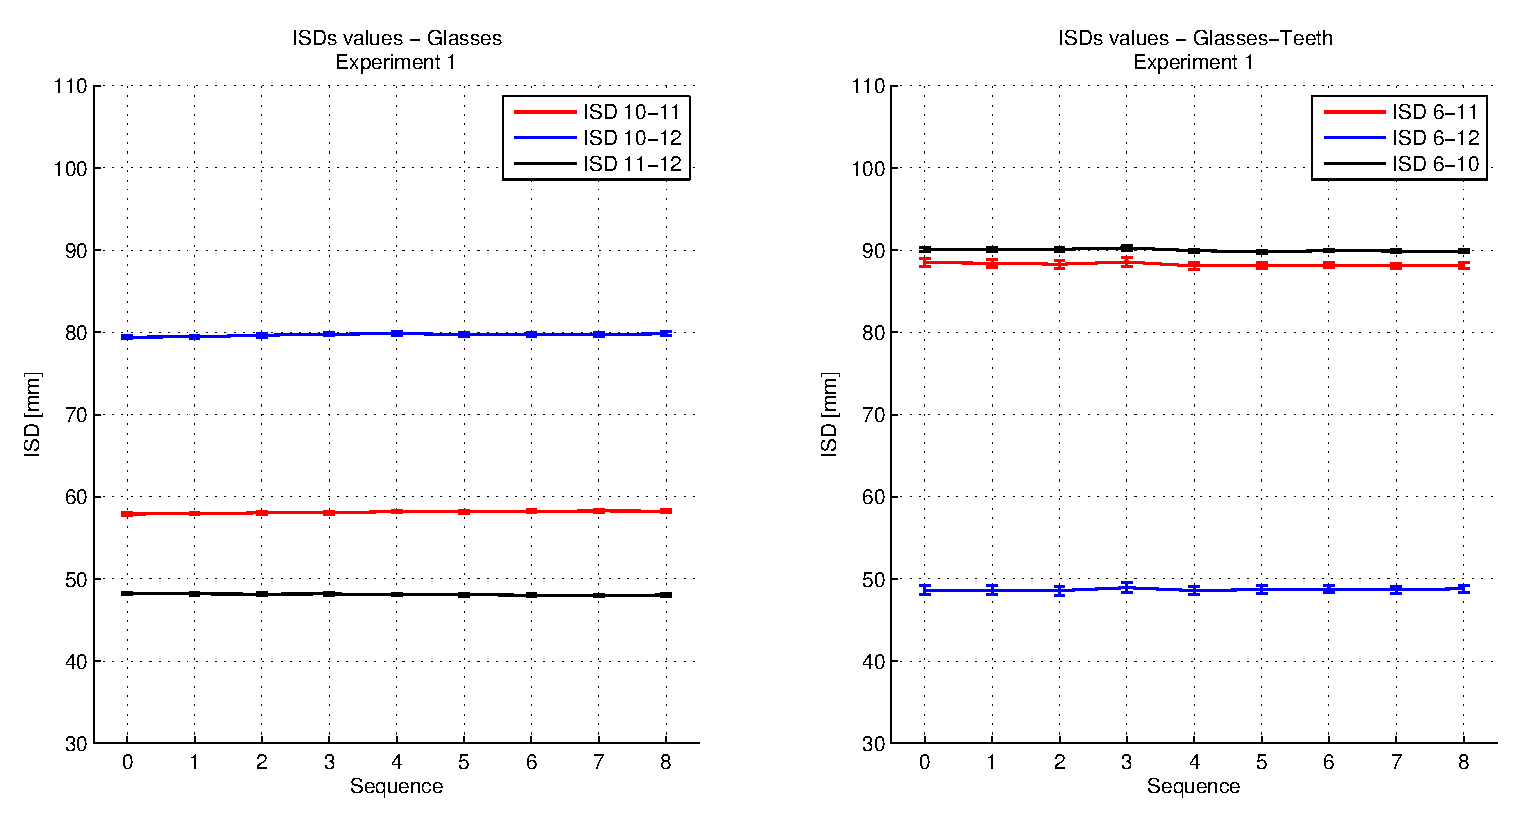
\includegraphics[width=0.75\textwidth]{include/linguometer/images/example_isd_1.eps}}
	\subfigure[\label{fig:linguometer:technical:isd:example:3}]
	{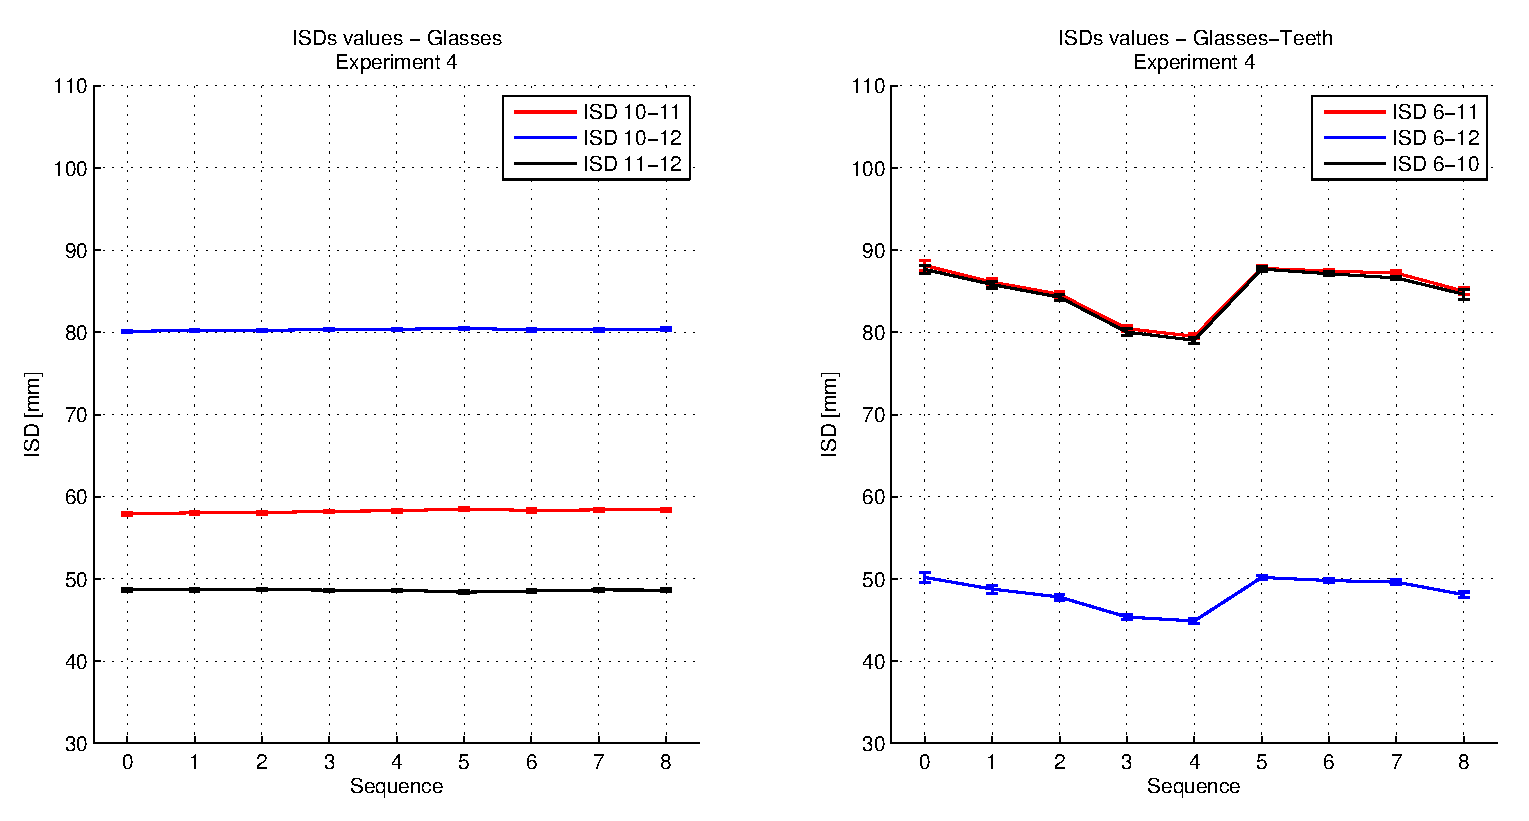
\includegraphics[width=0.75\textwidth]{include/linguometer/images/example_isd_4.eps}}
	\hspace{0.475\textwidth}
	
	\caption[ISD results (experiments)]{\textbf{ISD results
	(experiments)}: verification of
	the quality the kinesthetic data acquired by means of electromagnetic 
	articulography.
	The first plot (a) shows the results of a test experiment, where a sensor
	on the glasses (sensor 10) was left outside the spherical volume.
	}
	\label{fig:linguometer:technical:isd:example}
\end{figure}
% ---------------------------------------------------------------------------- %
